%%%%%%%%%%%%%%%%%%%%%%%%%%%%%%%%
\section{Results} \label{S:results}
%%%%%%%%%%%%%%%%%%%%%%%%%%%%%%%%
%
%###############################
\subsection{About our hypothesis} \label{sS:results_hypothesis}
%###############################
%
The current research used the Information-Theoretic Approach \citep{Anderson_2008, Chamberlain_1965} for model selection and inference. The application of the approach required: (i) the expression of the research hypothesis into statistical models, (ii) the selection of the most plausible models, and (iii) to produce inferences based on one or multiple selected models. The first requirement of the approach is covered in sections \ref{sS:causal_frame} and \ref{sS:stat_analysis}, and expanded in supplementary section \ref{sSA:model_details}. Here we use the results of the second requirement, detailed in the supplementary section \ref{ssSA:model_selection}, to produce the final inferences. 

As detailed in the aforementioned supplementary section, the final conclusions of our research will be drawn from the comparisons of two models: (i) a no interaction model, with one estimated `sample size' (model 3), and (ii) a full interaction model, with one estimated `sample size' (model 10). The former is selected as it is the model with highest probabilistic support. The latter is considered because it encompasses the remaining highest supported models. Furthermore, no \textit{robust} model is inspected, as we prefer a more parsimonious depiction of our hypothesis. Table \ref{tab:results} summarizes the parameters posterior estimates and contrasts of interest.
%
\begin{table}[h!]
	\centering
	\begin{tabular}{|cccccccccccc|} 
		\hline
		& \multicolumn{3}{c}{} & \multicolumn{2}{c}{CI} & & \multicolumn{2}{c}{HPDI} & & \multicolumn{2}{c|}{}\\[0.5ex]
		\cline{5-6} \cline{8-9}
		Parameter & Mean & SD & & $2.5\%$ & $97.5\%$ & & $2.5\%$ & $97.5\%$ & & n eff. & Rhat \\[0.5ex] 
		\hline\hline
		\rowcolor{gray}
		\multicolumn{12}{|l|}{ \textbf{Model 3: No interaction (one `size')} } \\
		\multicolumn{12}{|l|}{ \textbf{parameters:} } \\
		\texttt{a} & 0.179 & 0.189 & & -0.197 & 0.554 & & -0.198 & 0.552 & & 3677.705 & 1.001\\
		\texttt{bP[2]} & -0.117 & 0.166 & & -0.439 & 0.207 & & -0.440 & 0.202 & & 1738.855 & 1.000 \\
		\texttt{bA} & 0.432 & 0.141 & & 0.154 & 0.715 & & 0.170 & 0.723 & & 1815.243 & 1.001 \\
		\texttt{aHS[1]} & 0.284 & 0.235 & & -0.178 & 0.761 & & -0.203 & 0.728 & & 2719.833 & 1.000 \\
		\texttt{aHS[2]} & 0.116 & 0.217 & & -0.303 & 0.537 & & -0.304 & 0.537 & & 2646.671 & 1.000 \\
		\multicolumn{12}{|l|}{ \textbf{constrast:} } \\
		\texttt{aHS[2]-aHS[1]} & -0.168 & 0.246 & & -0.661 & 0.371 & & -0.650 & 0.324 & & n.a. & n.a. \\
		\multicolumn{12}{|l|}{ } \\
		\rowcolor{gray}
		\multicolumn{12}{|l|}{ \textbf{Model 10: Full interaction (one `size')} } \\
		\multicolumn{12}{|l|}{ \textbf{parameters:} } \\
		\texttt{a} & 0.217 & 0.179 & & -0.142 & 0.562 & & -0.118 & 0.580 & & 3902.629 & 0.999 \\
		\texttt{bP[2]} & -0.122 & 0.173 & & -0.457 & 0.220 & & -0.460 & 0.216 & & 1659.639 & 1.002 \\
		\texttt{bAHS[1]} & 0.435 & 0.157 & & 0.127 & 0.745 & & 0.123 & 0.741 & & 1477.460 & 1.000 \\
		\texttt{bAHS[2]} & 0.237 & 0.177 & & -0.119 & 0.596 & & -0.089 & 0.615 & & 1844.785 & 1.001 \\
		\texttt{aEHS[1,1]} & 0.183 & 0.278 & & -0.358 & 0.726 & & -0.349 & 0.729 & & 2524.451 & 1.000 \\
		\texttt{aEHS[2,2]} & 0.212 & 0.241 & & -0.259 & 0.684 & & -0.259 & 0.684 & & 2418.275 & 0.999 \\
		\texttt{aEHS[3,2]} & 0.077 & 0.245 & & -0.402 & 0.547 & & -0.383 & 0.561 & & 3015.559 & 0.999 \\
		\texttt{aEHS[4,2]} & 0.007 & 0.269 & & -0.522 & 0.530 & & -0.547 & 0.499 & & 3268.043 & 1.000 \\
		\multicolumn{12}{|l|}{ \textbf{contrast:} } \\
		\texttt{bAHS[2]-bAHS[1]} & -0.197 & 0.208 & & -0.600 & 0.213 & & -0.590 & 0.223 & & n.a. & n.a. \\
		\texttt{aEHS[2,2]-aEHS[1,1]} & 0.029 & 0.352 & & -0.673 & 0.723 & & -0.714 & 0.682 & & n.a. & n.a. \\
		\texttt{aEHS[3,2]-aEHS[1,1]} & -0.106 & 0.365 & & -0.823 & 0.607 & & -0.822 & 0.609 & & n.a. & n.a. \\
		\texttt{aEHS[4,2]-aEHS[1,1]} & -0.176 & 0.380 & & -0.906 & 0.568 & & -0.928 & 0.535 & & n.a. & n.a. \\
		\texttt{aEHS[3,2]-aEHS[2,2]} & -0.135 & 0.299 & & -0.719 & 0.453 & & -0.730 & 0.439 & & n.a. & n.a. \\
		\texttt{aEHS[4,2]-aEHS[2,2]} & -0.205 & 0.344 & & -0.888 & 0.453 & & -0.902 & 0.430 & & n.a. & n.a. \\
		\texttt{aEHS[4,2]-aEHS[3,2]} & -0.070 & 0.344 & & -0.744 & 0.612 & & -0.735 & 0.617 & & n.a. & n.a. \\
		\hline
		\multicolumn{12}{l}{\footnotesize{CI = compatibility interval}} \\
		\multicolumn{12}{l}{\footnotesize{HDPI = highest posterior density interval}} \\
		\multicolumn{12}{l}{\footnotesize{n eff. = effective number samples}} \\
		\multicolumn{12}{l}{\footnotesize{Rhat = Gelman-Rubin diagnostic}} \\
		\multicolumn{12}{l}{\footnotesize{n.a. = not available / not applicable}} \\
		\multicolumn{12}{l}{\footnotesize{[1] = NH children, [2] = HI/CI children}} \\
		\multicolumn{12}{l}{\footnotesize{[1,i] = NH children, [2,i] = genetic, [3,i] = CMV infection, [4,i] = unknown etiology}} \\
	\end{tabular}
	\caption[Selected statistical models: results]{Selected statistical models: results.}
	\label{tab:results}
\end{table}

Before any interpretation of the parameters, it is important to highlight a problematic that will permeate all of our inferences. Given the large amount of variability registered at the children and replicates levels, the models will not be able to produce unequivocal null hypothesis rejections (compatibility and HPD intervals not including zero). The reasons for this are further expanded in section \ref{sS:results_variability}. However, from supplementary section \ref{ssSA:model_simulation}, we can be certain that our models can affirm the parameter values with at least $60\%$ power, depending on the size of the effects. Therefore we will continue interpreting the parameters, but the reader should cautious into understand the CI and HPDI indicate our data size is not enough to ultimately define the conclusions here arrived.

First, about \textbf{\textit{hearing status}}, model three reveals that HI/CI children have a modest lower level of \textit{speech intelligibility}, compared to their NH counterparts (\texttt{aHS[2]-aHS[1]}). The result then seem to support previous evidence on the matter \cite{Nicholas_et_al_2007, Castellanos_et_al_2014, Chin_et_al_2014, Geers_et_al_2016, Freeman_et_al_2017, Duchesne_et_al_2019, Grandon_et_al_2020}. 

However, model ten paints a more nuanced story. The contrasts of the model reveal that HI/CI children with genetic etiology manage to reach similar levels of \textit{intelligibility} as NH children (\texttt{aEHS[2,2]-aEHS[1,1]}), but the same cannot be said when the hearing impairment is caused either by a CMV infection (\texttt{aEHS[3,2]-aEHS[1,1]}) or other unknown causes (\texttt{aEHS[4,2]-aEHS[1,1]}). The former result seem intuitive, as children with genetic causes have grown developing their language using the hearing apparatus, and therefore, also developing the appropriate neural connections to benefit from the new hearing input from the start, even when that input is slightly degraded \cite{Drennan_et_al_2008}. In contrast, the evidence seem to suggest a different scenario for HI/CI children with other etiology status. What is hinted is that a child with other etiology status might need to `rewire' his(her) neural connection in order to fully take advantage of the new hearing input signal, as it is assumed they begin their life hearing normally, and then loosing the ability to process sound. This result is particularly important, as it reveals that the factors that caused the hearing impairment matter, even when the children receive the new hearing input signal at a young age.

%
\begin{comment}
About \textbf{\textit{hearing age}} ($A_{i}$), we expect it to be one of the main responsible for the increase in children's \textit{speech intelligibility}, no mater the children's hearing status \cite{Boonen_et_al_2021}. \textit{Hearing age} is a composite variable constructed by combining the \textit{chronological age} for the NH group, and the \textit{device length of use} for the HI/CI group \citep{Faes_et_al_2021} (see table \ref{tab:characteristics}). The variable tries to approximate the amount of time a child has been actively hearing and developing his(her) language. 

Several studies provide evidence that intelligibility increases with age \cite{Chin_et_al_2001, Chin_et_al_2003, Flipsen_2006, Flipsen_2008, Baudonck_et_al_2009, Bowen_2011, Hustad_et_al_2020}, and no short of evidence has been presented in favor of using others surrogate measures, like \textit{chronological age} \cite{Flipsen_et_al_2006, Habib_et_al_2010, Grandon_et_al_2020} or \textit{age at implantation} \cite{Niparko_et_al_2010, Boons_et_al_2012, Bruijnzeel_et_al_2016, Dettman_et_al_2016}. We argue that the feasibility of using any other proxy measure, largely depends on the assumed reliability of the surrogate to approximate the variable of interest. In that sense, although we recognize \textit{hearing age} is not a `perfect' proxy \cite{Faes_et_al_2021}, we argue it is the most appropriate to test our hypothesis, based on the relevant literature review and its assumed reliability to capture children's language development (although the latter has not been tested). Furthermore, we believe the variable serve two additional purposes: (i) control for sampling bias (expanded in supplementary section \ref{sSA:sampling_bias}), and (ii) de-confound the parameter estimates of \textit{hearing status} \cite{Cinelli_et_al_2021}.

Finally, it is important to highlight that for modeling purposes, using more than one of the aforementioned proxies in tandem is not recommended. It is apparent from the previous description, the three surrogate measures share high similarities in their data construction. This in turn, could cause problems in the modeling procedure, as including variables that provide `similar information' might lead to a statistical problem known as multicollinearity, in which our estimates get biased and less precise \cite{Farrar_et_al_1967}, leading us to incorrect inferences and conclusions.

For \textbf{\textit{pure tone average}} ($PTA_{i}$), we expect it to have a small or null effect on \textit{speech intelligibility}, as the empirical evidence seem to suggest \cite{Boonen_et_al_2021}. \textit{Pure tone average} is the child's subjective hearing sensitivity, aided or unaided, by their hearing apparatus. 

However, beyond the empirical evidence, the variable was included for two additional reasons. First, given that previous modeling efforts did not capture the full data hierarchy, it is possible that the effects of PTA on \textit{speech intelligibility} has been largely overlooked. Although evidence seem to suggest the variable has no effect, it is also sensible to think that HI/CI children with severe hearing loss, as accounted by the variable, might develop their language at a slower rate. This is especially true, if we consider the signal provided by the cochlear implant is still degraded compared to normal hearing scenarios \cite{Drennan_et_al_2008}. Lastly, a second reason is that the variable might be useful to de-confound the parameter estimates of \textit{hearing status} \cite{Cinelli_et_al_2021}, a purpose shared with the variable \textit{hearing age}. 

In the case of the \textbf{\textit{Etiology}} of the disease that led to the hearing impairment ($E_{i}$), we expect it to have a differential effect on \textit{speech intelligibility}, within the HI/CI group. However, since the severity of the etiology cannot be easily ascertain nor ordered, we cannot foresee the direction of such effects, i.e. genetic factors not necessarily lead to worse levels of language development and intelligibility, than factors related to infections.

The previous assumption does not have a correspondence with the empirical evidence, were the variable was deemed unimportant \cite{Boonen_et_al_2021}. However, we argue that it is possible its effects have also been largely overlooked, due to the lack of statistical control of the full data hierarchy, similar to the PTA case. Moreover, as with its predecessors, the variable might also be useful to de-confound the parameter estimates of \textit{hearing status} \cite{Cinelli_et_al_2021}, assuming our DAG is appropriate.
\end{comment}
	
\textcolor{red}{work in progress}

\begin{comment}
“simplest” model (E_NC2b) provides
(preliminar) evidence on,
the higher the unaided PTA the
lower the child’s SI (bP[2])
(based on power analysis, we can be
sure is a small effect)
no apparent statistical difference
between NH and HI=CI children
(but this requires a CONTRAST)
for each “hearing” year, the SI
increases in approx 0:40 logits
(effect larger than the assumed in
power analysis)

however, the “interaction” model
(E_NC5b3) shows similar results on,
the small (still non-significant)
effects of the unaided PTA on the
child’s SI
similar explained variability across
levels and blocks
(similar to the “simplest” model)
but “mild” evidence of prevalent
interactions,
SI means for HI=CI per E,
aEHS[2; 2] (Genetic) vs
aEHS[3; 2] (CMV)
different SI evolution for NH vs
HI=CI children, per unit A
(bAHS),

within the “interaction” model,
the size of the data within groups
from combinations of E and HS,
does not allow to reject the
contrasts’ null hypothesis,
similar result is observed on the
bAHS contrast
(because the effect is small, compared
to children’s variability)
but we still observe differences
between NH and HI/CI, and even
within HI/CI by E,
therefore we decide to keep the
(E_NC5b3) model
\end{comment}
%
%
%###############################
\subsection{About the hierarchy of variability} \label{sS:results_variability}
%###############################
%
As expected, three hierarchies of variability were present in our data: the blocks and children's random effects, as well as, the variability of the entropy replicates.

Evidence from the posterior estimates reveal the block random effects explained a small amount of variability in the data (top panel of figure \ref{fig:variability}), and its inclusion/exclusion in the model did not change the parameter estimates. The previous implies the experiment was correctly `set up', as the series in which the utterances were transcribed did not explain a significant amount of variation, nor its exclusion biased the parameter estimates.

On the contrary, we observe a significantly larger variability between children's \textit{speech intelligibility}, more precisely, more than three times the block effects variability (middle panel of figure \ref{fig:variability}). The previous corroborated preliminary evidence on the matter \cite{Young_et_al_2002, Peng_et_al_2004, Montag_et_al_2014, Castellanos_et_al_2014, Yanbay_et_al_2014, Nittrouer_et_al_2014, Freeman_et_al_2017, Boonen_et_al_2021}. Additionally, it implied that given such a large amount of between variability, the statistical models might have a harder time delimiting the \textit{hearing status} groups location on the intelligibility scale.

Finally, for the variability of the entropy replicates, the posterior estimates reveal a reasonable finding: the amount of variability at the replicates level is even larger than the one observed at the children level (bottom panel of figure \ref{fig:variability}). The latter implies there is significant error in measuring speech intelligibility with the entropy replicates. This further emphasize the difficulty of producing unequivocal  inferences, in respect to the intelligibility levels of the \textit{hearing status} groups.
%
\begin{figure}[!h]
	\centering
	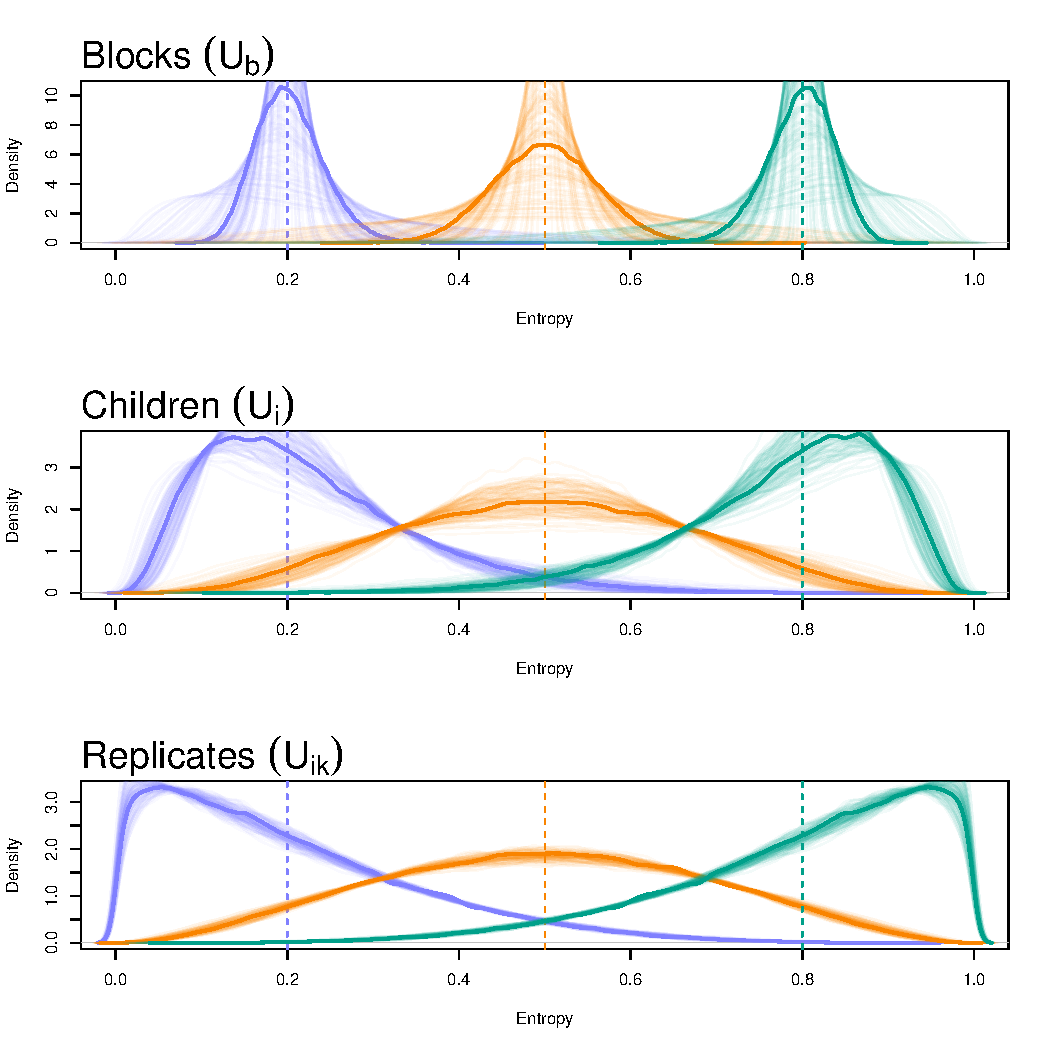
\includegraphics[width=0.6\linewidth]{variability_plot.pdf}
	\caption[Posterior predictive: hierarchy of variability in the data]{Posterior predictive: hierarchy of variability in the data. Distributions are plotted at the entropy replicates scale, considering three different average entropy values: $\mu=0.2$, $\mu=0.5$, and $\mu=0.8$ (discontinuous lines). Thick solid lines represent the marginal distribution, thin solid lines depict $100$ random posterior samples.}
	\label{fig:variability}
\end{figure}
%
%
%###############################
\subsection{The speech intelligibility scale} \label{sS:results_scales}
%###############################
%
\textcolor{red}{work in progress}
%
\begin{figure}[!h]
	\centering
	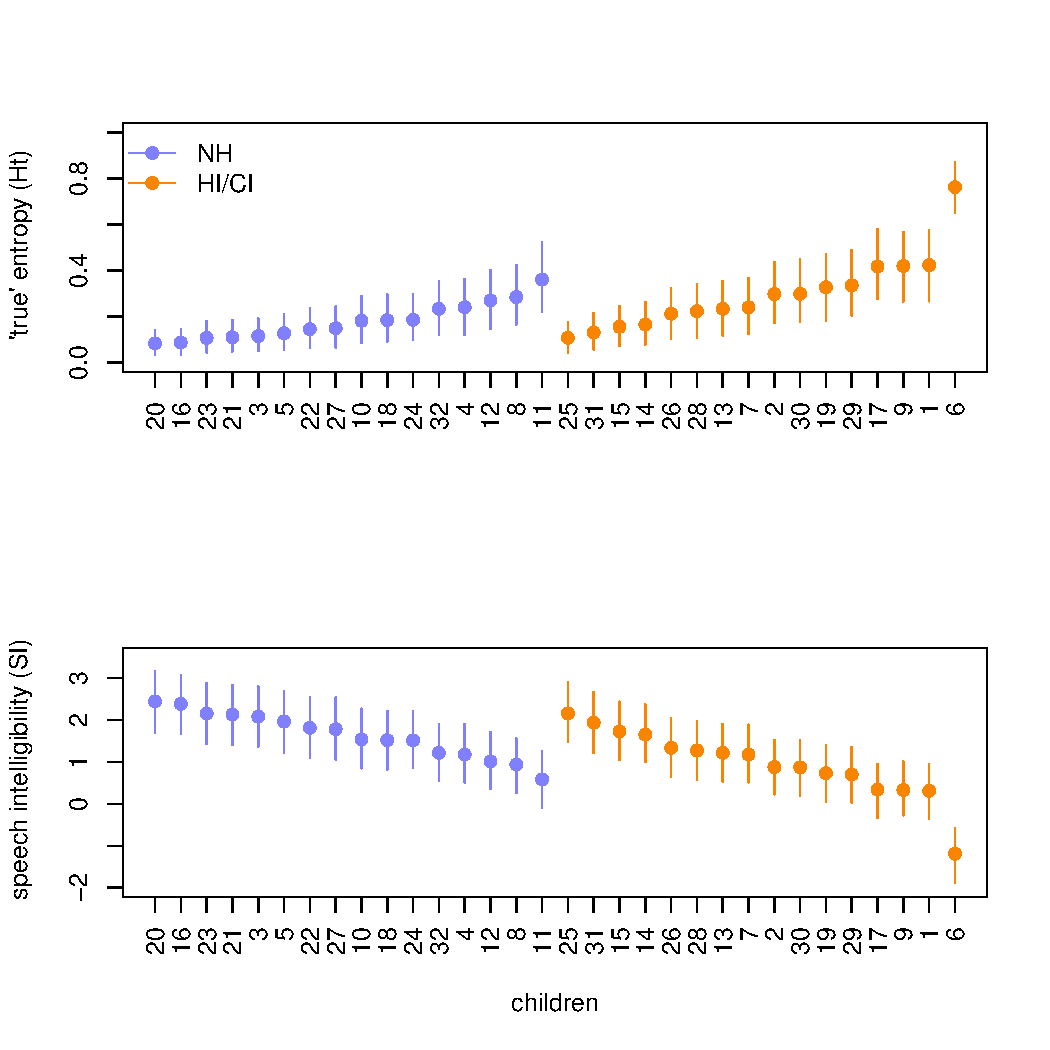
\includegraphics[width=0.7\linewidth]{posterior_predictive_real2.pdf}
	\caption[Posterior predictive: \textit{true} entropy and \textit{speech intelligibility} scales]{Posterior predictive: \textit{true} entropy and \textit{speech intelligibility} scales. Circles represent mean values, lines depict $95\%$ highest posterior density intervals (HDPI). Horizontal discontinuous lines represent the marginal average for the \textit{hearing status} group.}
	\label{fig:predictive2}
\end{figure}
%
%
%###############################
\subsection{Posterior predictive} \label{sS:results_posterior}
%###############################
%
\textcolor{red}{work in progress}
%
\begin{figure}[!h]
	\centering
	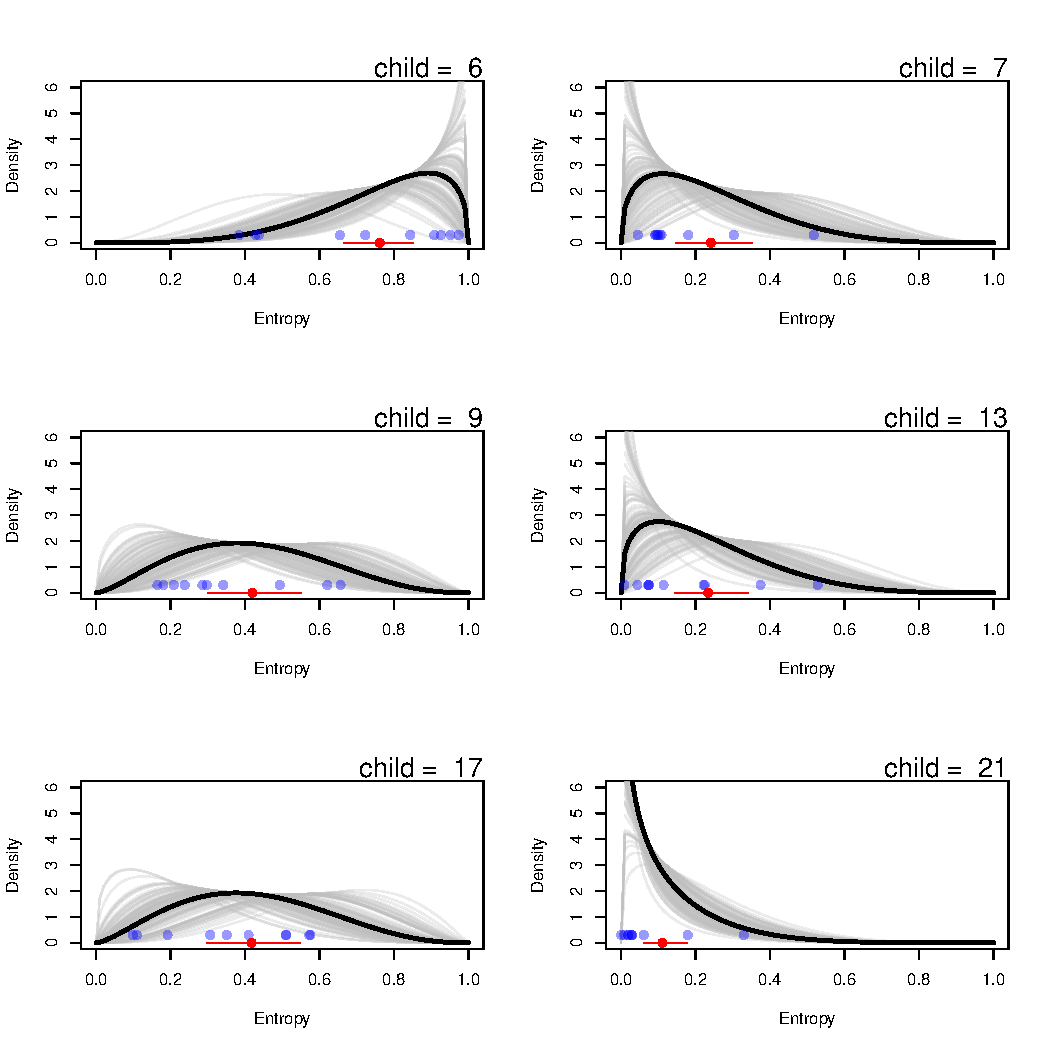
\includegraphics[width=0.7\linewidth]{posterior_predictive_real1.pdf}
	\caption[Posterior predictive: entropy replicates]{Posterior predictive: entropy replicates. Red point with lines represent the mean \textit{true} entropy with $95\%$ highest posterior density interval (HPDI). Thick solid line represents the marginal distribution, thin solid lines depicts $100$ random posterior samples.}
	\label{fig:predictive1}
\end{figure}
%
%
%###############################
\subsection{Influential observations} \label{sS:results_outliers}
%###############################
%
\textcolor{red}{work in progress}
%
\begin{figure}[!h]
	\centering
	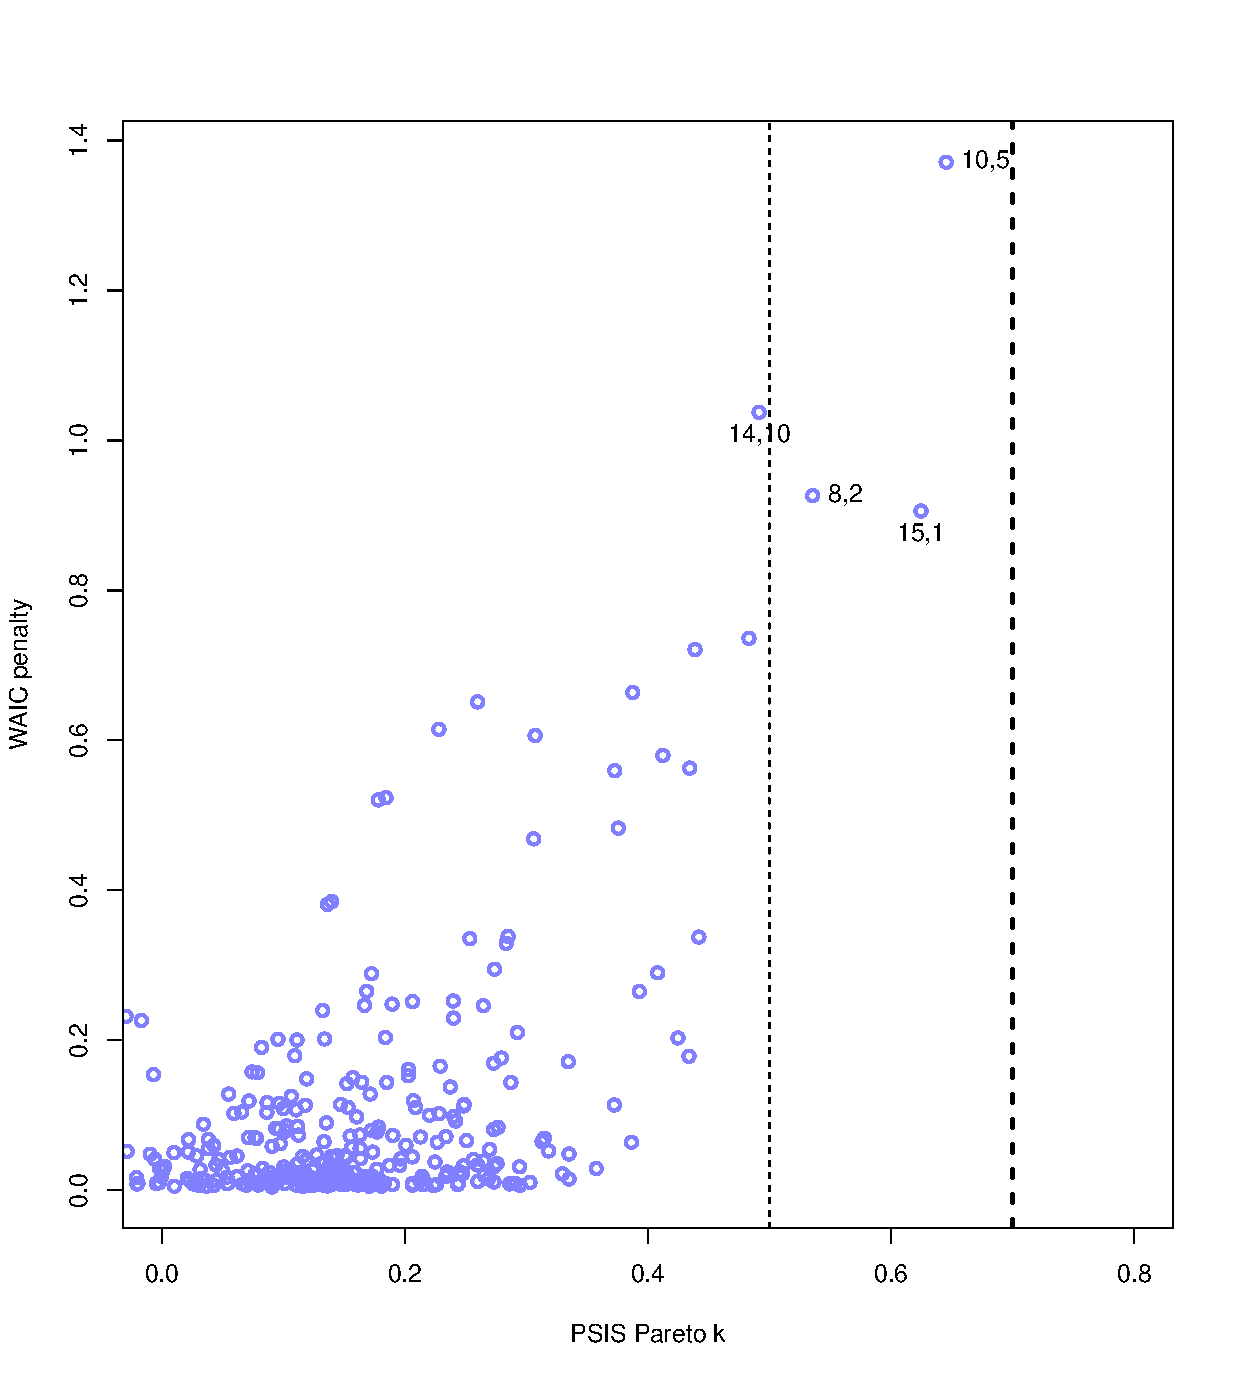
\includegraphics[width=0.5\linewidth]{outliers.pdf}
	\caption[Influential observations]{Influential observations. Pairs (child, utterance) are reported for specific observations.}
	\label{fig:outliers}
\end{figure}
%
%